%%%%%%%%%%%%%%%%%%%%%%%%%%%%%%%%%%%%%%%%%%%%%%%%%%%%%%%%%%%%%%
% --> ENUNCIADO
%%%%%%%%%%%%%%%%%%%%%%%%%%%%%%%%%%%%%%%%%%%%%%%%%%%%%%%%%%%%%%
\section{Enunciado}
El objetivo de este proyecto es familiarizar al estudiante con la programación forma de una estructura de datos básica y/o algoritmo en el lenguaje C++, así como su análisis y presentación. Particularmente en este proyecto se crearan imágenes digitales a partir de archivos binarios.

Se deben tomar archivos binarios de cualquier  índole y calcular el tamaño máximo que puede crearse con sus bytes una imagen X × Y píxeles (no necesariamente cuadrada), tomando en cuenta que cada píxel de dicha imagen esta representado por 3 bytes que representan intensidad de colores rojo, verde y azul, cuyos valores varían entre 0 y 255. Su programa debe tener la capacidad de escribir imágenes en formatos PNG, JPEG, GIF, BMP. Puede utilizar bibliotecas de terceros para implementar esta ultima funcionalidad.
%%%%%%%%%%%%%%%%%%%%%%%%%%%%%%%%%%%%%%%%%%%%%%%%%%%%%%%%%%%%%%
% --> RESEÑA DEL ALGORITMO/ESTRUCTURA
%%%%%%%%%%%%%%%%%%%%%%%%%%%%%%%%%%%%%%%%%%%%%%%%%%%%%%%%%%%%%%
\section{Reseña del algoritmo/estructura}

Una imagen digital en formato RGB se forma por combinación de tres canales. Cada canal se corresponde con un color primario: Red (rojo), Green (verde), y Blue (azul), en donde se asigna un valor de intensidad a cada color que oscila entre 0 y 255, por lo que cada valor de color debe ser guardo en 8 bits o un byte. De la combinación surgen hasta 16,7 millones de colores, que son capaces de describir la mayoría de las imágenes a nivel digital.

En la figura \ref{fig:matrizRGB}, se puede observar con mayor claridad este concepto.

\begin{figure}[H]
\centering
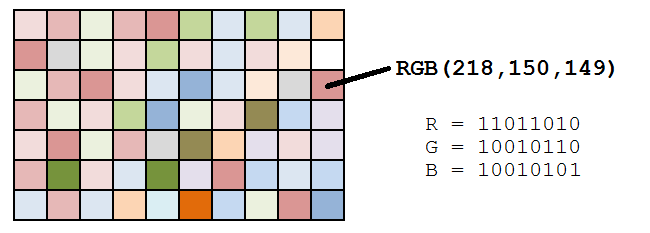
\includegraphics[width=0.6\textwidth]{imgs/proyecto0/matrix.png}
\caption{Imágenes en formato PNG}
\label{fig:matrizRGB}
\end{figure}

Existen en la actualidad una gran cantidad de formatos de archivo que permiten visualizar imágenes digitales que utilizan el mapeo RGB. Esto permite que sea posible implementar algún método que convierta un archivo binario, extrayendo su información en forma de bits puros, mapearlo a RGB, y presentarlo en uno de estos  estándar, de manera que se pueda visualizar con algún dispositivo digital capaz de abrir la imagen. Entre los estándares más comunes se encuentran BMP, PNG, JPG y GIF.

%ESTO SUENA RARO, VOY A TRATAR DE REFRASEARLO   Para generar estas imágenes a partir de un archivo binario de 1 y 0, existen en la actualidad una gran cantidad de formatos de imágenes que nos permite pasar de un archivo binario a una imagen con un formato estándar el cual se puede visualizar con algún dispositivo digital capaz de abrir la imagen con un formato especifico>>> NO LO SÉ, RICK. Entre los estándares más comunes se encuentran BMP, PNG, JPG y GIF. 

A continuación se presenta una breve descripición de las características básicas de los distintos formatos de imagénes que se pretenden usar en este proyecto:

\begin{itemize}
    \item \textbf{PNG}: Las imágenes \textit{Portable Network Graphics}, según \cite{R2} es un formato de imagen sin pérdida que se publicó en 1996. PNG no se diseñó para uso profesional, sino para transferir imágenes en Internet, y solo admite imágenes de nivel de grises e imágenes rgb (también imágenes de color basadas en paletas).
    %---------------------------------------------------------------------
    \item \textbf{JPEG}: Los archivos en formato \textit{Joint Photographic Experts Group}, según \cite{R2} es un formato de imagen que fue aprobado como estándar internacional en 1994. JPEG es usualmente con pérdida, pero también puede ser sin pérdida y se ha convertido en un formato popular para la representación de imágenes en Internet. El estándar define tanto los algoritmos para codificar y decodificar como formato de almacenamiento. JPEG divide la imagen en bloques de 8 × 8 y transforma cada bloquear con una Transformada de Coseno Discreta. Estos valores corresponden a valores más altos 359 frecuencias (variaciones rápidas de color) se establecen en 0 a menos que sean bastante grande, ya que esto no se nota mucho por la percepción humana. Los valores DCT perturbados luego están codificados por una variación de la codificación de Huffman. JPEG también puede usar aritmética codificación, pero esto aumenta los tiempos de codificación y decodificación, con solo alrededor del $\percent[5]$ de mejora en la relación de compresión. El nivel de compresión en imágenes JPEG es seleccionado por el usuario y puede resultar en artefactos conspicuos
    si está configurado demasiado alto. JPEG es especialmente propenso a artefactos en áreas donde la intensidad cambia rápidamente de píxel a píxel. La extensión de un archivo JPEG es .jpg o .jpeg
    %---------------------------------------------------------------------
    \item \textbf{GIF}: El formato \textit{Graphics Interchange Format} fue desarrollado en 1987 por CompuServe Incorporated, principalmente para su uso en Internet. Según \cite{R3}, este formato admite profundidades de color de 1 bit (monocromo) a 8 bits (256 colores) y almacena siempre las imágenes en forma comprimida, utilizando compresión LZW sin pérdida. Otras características compatibles incluyen entrelazado y transparencia.
    %---------------------------------------------------------------------
    \item \textbf{BMP}: El formato \textit{BitMap} fue desarrollado por Microsoft como el formato nativo del sistema operativo Windows. Las versiones del formato han coincidido con las versiones de Windows, la primera versión que aparece en 1985 con Windows 1.0. Según \cite{R3} es un formato  que admite profundidades de color de 1 bit a 32 bits y proporciona compresión RLE opcional sin pérdida.
\end{itemize}

En el cuadro \ref{T:T111}, se muestra un resumen de los distintos formatos: 

\begin{table}[H]
\begin{center}
    \begin{tabular}{ |>{\centering\arraybackslash}m{4cm}|>{\centering\arraybackslash}m{5.5cm}|>{\centering\arraybackslash}m{5.5cm}| }
    	\hline
    	\cellcolor{cl} \textbf{Formato} & \cellcolor{cl} \textbf{Ventajas} & \cellcolor{cl} \textbf{Desventajas}\\ \hline \hline
    	PNG (\textit{Portable Network Graphics}) & Es mejor cuando la imagen tiene grandes áreas uniformemente coloreadas; robusto& Muchos navegadores antiguos actualmente no son compatibles con el formato de archivo PNG. \\
    	\hline
    	JPEG (\textit{Joint Photographic Experts Group}) & Pequeños archivos: la compresión no afecta de manera apreciable la calidad de la imagen & - \\
    	\hline
    	GIF (\textit{Graphics Interchange Format}) & Soporta animaciones & Limitado a 256 colores, sin función real en comparación con otros formatos.\\
    	\hline
    	BMP (\textit{BitMap}) &Son ampliamente usados en los programas de Windows&Son archivos grandes y sin comprimir.\\
    	\hline
    \end{tabular}
\end{center}
\label{T:T111}
\caption{Resumen de características de los formatos de imágenes. \cite{R1}}
\end{table}


%%%%%%%%%%%%%%%%%%%%%%%%%%%%%%%%%%%%%%%%%%%%%%%%%%%%%%%%%%%%%%
% --> FUNCIONAMIENTO DEL ALGORITMO
%%%%%%%%%%%%%%%%%%%%%%%%%%%%%%%%%%%%%%%%%%%%%%%%%%%%%%%%%%%%%%
\section{Funcionamiento del algoritmo/estructura}
El programa constará de varias clases y métodos para la lectura, traducción y escritura. Se utilizará una estructura de herencia, donde se tendrán las siguientes clases y métodos:
%------------------------------
\subsection{Clase Base Píxeles}
%------------------------------
Esta clase contendrá un método encargado de leer un archivo .txt con la ruta del archivo de entrada que contiene los datos en binario del código que se quiere representar mediante una imagen. Con este código también se calcula el tamaño en bytes del archivo de entrada, para esto se utilizará una biblioteca como \texttt{fstream} con su método \texttt{read()}, o bien utilizando la función \texttt{stat} de la biblioteca \texttt{sys/stat.h}. Una vez se tenga lo anterior, se almacenarán los datos de la hilera de entrada en un arreglo o vector, sobre el cual se trabajará. Por tal razón, es posible que esta clase cuente con los siguientes métodos:

    
\begin{itemize}
    %\item \textbf{Clase base:} 
    %Esta clase contendrá un método encargado de leer un archivo .txt con la ruta del archivo de entrada que contiene los datos en binario del código que se quiere representar mediante una imagen. Con este código también se calcula el tamaño en bytes del archivo de entrada, para esto se utilizará una biblioteca como \texttt{fstream} con su método \texttt{read()}, o bien utilizando la función \texttt{stat} de la biblioteca \texttt{sys/stat.h} \cite{R7}. Una vez se tenga lo anterior, se almacenarán los datos de la hilera de entrada en un arreglo o vector, sobre el cual se trabajará. 
    \item \textbf{Método de formato:} 
    Esta función tomará el arreglo a trabajar y calculará si tiene el tamaño suficiente para generar una imagen, además definirá la relación de aspecto de la imagen . Los formatos a utilizar serán los más comunes, como lo son 16:9, 4:3, 3:2 y 1:1. En caso de que se tenga una cantidad suficiente de bytes para generar la imagen, pero falten o sobren datos, se truncará el arreglo, y se eliminarán los últimos bytes de éste.
    \item \textbf{Método del algoritmo de traducción:} Esta función será la más importante debido a que es la encargada de traducir de un binario a una imagen. Para la traducción se utilizará el modelo RGB, en donde las imágenes son representadas por los colores rojo, verde y azul. Cada uno de estos colores se representa con un número binario que va de 0 a 255 en base decimal, o en binario, de 00000000 a 11111111 \cite{R5}. El valor más bajo representa la tonalidad más oscura del color, y el valor más alto representa la tonalidad más clara. Para la traducción se tomará el arreglo y se analizará, bloques de 24bits, o lo que es lo mismo, 3 bytes consecutivos. Cada triada se tomará de manera que los primeros 8 bits en binario sean la tonalidad de rojo; los siguientes 8 bits la tonalidad verde y los siguientes la tonalidad en azul. Cada triada con sus respectivos tres valores RGB corresponde a un píxel de la imagen. Una vez que se completa la traducción, el método devuelve un arreglo o hilera RGB listo para su representación visual.
    %\item \textbf{Generación de la imagen:} 
\end{itemize}

%Las clases derivadas deben ser capaces 

%------------------------------
\subsection{Clase Derivada BMP} 
%------------------------------

Esta clase debe ser capaz de tomar el unsigned char *rgb o el archivo binario ya convertido en formato RGB y guardarlo en una ruta especificada por la string filename. Según la investigación realiada, para lograr esto se deben definir los atributos necesarios del header de un archivo en formato BMP y además esta clase debe ser capaz de lograr al menos el siguiente método:
 
\begin{itemize}
    \item \textbf{Método guardar array RGB en formato BMP}: este método debe ser capaz de tomar los atributos de esta clase y hacer uso de la función \texttt{fwrite()}, lograr escribir la imagen en formato BMP.
\end{itemize}

En este caso no es necesario usar una biblioteca de terceros, ya que todas las funciones necesarias se encuentran dentro de las librería estandar de C++, esto se puede ya que este formato no hace de ningún método de comprensión de los datos para generar la imagen. 

%------------------------------
\subsection{Clase Derivada PNG}
%------------------------------

Esta clase contiene funciones capaces de trabajar el formato PNG. Para esto se puede utilizar la biblioteca \texttt{libpng}.

\begin{itemize}
    \item \textbf{Método guardar array RGB en formato PNG}: este método debe ser capaz de abrir en el archivo RGB del espacio de trabajo mediante un puntero, debe crear la imagen y guardarla.
\end{itemize}

% PNG -> libpng-dev -> sudo apt-get install libpng-dev \cite{R6}

%------------------------------
\subsection{Clase Derivada JPEG}
%------------------------------
Esta clase contiene funciones capaces de trabajar el formato JPEG con su algoritmo de compresión. Para esto se puede utilizar la biblioteca \texttt{libjpeg}, toda esta biblioteca está escrita completamente en C, por lo que su uso en C++ no debe de generar problemas.

\begin{itemize}
    \item \textbf{Método guardar array RGB en formato JPEG}: este método debe ser capaz de abrir en el archivo RGB del espacio de trabajo mediante un puntero y aplicarle la compresión de acuerdo a la calidad deseada. Al final debe crear la imagen y guardarla.
\end{itemize}

% PNG -> libjpeg-dev -> sudo apt-get install libjpeg-dev 

%------------------------------
\subsection{Clase Derivada GIF}
%------------------------------
Para implementar las funcionalidades de esta clase se puede utilizar la biblioteca \texttt{Magick++}. Ésta es parte del paquete \texttt{ImageMagick}, y provee una muy amplia gama de clases y métodos para trabajar con imágenes, y soporta gran cantidad de formatos. En este caso, nos interesa generar una imagen en formato GIF a partir del arreglo de pixeles obtenido anteriormente.

Otra alternativa es utilizar la biblioteca \texttt{giflib}, que permite convertir directamente imágenes en formato GIF a tripletas RGB de 24 bits y viceversa \cite{R8}.

\begin{itemize}
    \item \textbf{Método guardar array RGB en formato GIF}: Si se utiliza la herramienta \texttt{Magick++}, es posible crear un objeto de la clase \texttt{Image}, pasándole como parámetros sus dimensiones, el formato de mapeo de los pixeles (en este caso, RGB), el tipo de dato que guarda los pixeles (float, char, integer...) y el arreglo de datos que generará la imagen \cite{R9}. 
\end{itemize}

%%%%%%%%%%%%%%%%%%%%%%%%%%%%%%%%%%%%%%%%%%%%%%%%%%%%%%%%%%%%%%
% --> EXPERIMENTOS QUE SE REALIZARAN
%%%%%%%%%%%%%%%%%%%%%%%%%%%%%%%%%%%%%%%%%%%%%%%%%%%%%%%%%%%%%%
\section{Experimentos que se realizarán}


Para comprobar la funcionalidad del programa se ejecutará varias veces con diferentes entradas. En donde se variará el largo del archivo binario para comprobar cómo responde y cómo maneja casos especiales como no tener una cantidad suficiente de bytes, también se probará la respuesta ante posibles casos de error como si se presentase un símbolo diferente a un 1 o un 0. 

Otra de las pruebas a realizar corresponde a generar desde un mismo archivo imágenes con diferentes dimensiones, si se tiene la cantidad suficiente de datos.

Un caso importante que experimentar es utilizar como base el mismo archivo binario para crear una imagen de las mismas dimensiones pero en cada uno de los distintos formatos BMP, JPEG, GIF y PNG, y así observar si se obtiene la misma imagen de salida o si se obtiene un resultado distinto.



%%%%%%%%%%%%%%%%%%%%%%%%%%%%%%%%%%%%%%%%%%%%%%%%%%%%%%%%%%%%%%
% --> BIBLIOGRAFIA
%%%%%%%%%%%%%%%%%%%%%%%%%%%%%%%%%%%%%%%%%%%%%%%%%%%%%%%%%%%%%%
\begin{thebibliography}{IEEE}
\bibitem{R1} Luca, M. \textbf{\textit{A Basic Summary of Image Formats}}.  Visto el 5 de Mayo del 2018 en: \url{http://www.student.montefiore.ulg.ac.be/~merciadri/docs/papers/image-formats.pdf}.

\bibitem{R2} Autor Desconocido. \textbf{\textit{Digital images and image formats}}. Visto el 5 de Mayo del 2018 en: \url{http://www.uio.no/studier/emner/matnat/math/MAT-INF1100/h08/kompendiet/images.pdf}.

\bibitem{R3} Brown, A. \textbf{\textit{Graphics File Formats}}. 2008. THe National Archives. Visto el 5 de Mayo del 2018 en: \url{https://www.nationalarchives.gov.uk/documents/graphic-file-formats.pdf}.

\bibitem{R4} PNG. \textit{\textbf{Official documentation of libpng}}. Visto el 5 de Mayo del 2018 en: \url{http://www.libpng.org/pub/png/libpng.html}. 

\bibitem{R5} Kumar, T. Verma, K. \textbf{\textit{A Theory Based on Conversion of RGB image to Gray
image}}. 2010. International Journal of Computer Applications, Vol. 7. No. 2. Visto el 5 de Mayo del 2018 en: \url{https://www.researchgate.net/profile/Karun_Verma/publication/46286639_A_Theory_Based_on_Conversion_of_RGB_image_to_Gray_image/links/5704a3b008ae44d70ee0662c.pdf}.

\bibitem{R6} Greensted, A. \textbf{\textit{Creating PNGs with libpng}}. Visto el 5 de Mayo del 2018 en: \url{http://www.labbookpages.co.uk/software/imgProc/libPNG.html}.

\bibitem{R7} Autor Desconocido. \textbf{\textit{C++ Binary File I/O}}. Visto el 5 de Mayo del 2018 en: \url{http://courses.cs.vt.edu/~cs2604/fall00/binio.html}

\bibitem{R8} Raymon, E. \textbf{\textit{Introduction to GIFLIB}}. Visto el 5 de Mayo del 2018 en: \url{http://giflib.sourceforge.net/intro.html}

\bibitem{R9} Autor desconocido. \textbf{\textit{Magick::Image Class}}. Visto el 5 de Mayo del 2018 en: \url{https://www.imagemagick.org/api/Image++.php}



\end{thebibliography}